\section{Human pose estimation}

To interact with computers humans have come up with a plethora of methods. Ranging from early punch cards to modern touch screens, the methods have evolved to be more natural and intuitive. In recent years, the use of cameras to interact with computers has become more popular, since they require no physical contact and can make the use of computer systems seamless when developed properly.

In this section, REPLACE_WE discuss some of the methods that have been used to extract the pose of a human from videos of different formats. REPLACE_WE also discuss possible applications of human pose estimation. Finally, REPLACE_WE 

In chapter \ref{sec:errors} Human Pose Estimation Difficulties, REPLACE_WE go into more detail about the method REPLACE_WE used to extract the pose and what factors influence the result of the pose estimation.

We will go into more detail about some of the state-of-the-art human pose estimators for both RGB and RGBD data and even from point clouds in Section \ref{sec:related_work} Related Work.

\subsection{Pose visualisation}

There are mainly three different ways the human pose can be visualised. The first and most basic way is to visualise the pose as a skeleton. This is the most common way to visualise the pose of a human. The skeleton is made up of joints, which are connected by bones. The number of joints and bones can vary, but the most common skeleton is made up of 17 joints and 16 bones, as can be seen in Figure \ref{fig:pose_example}. The joints are usually labeled with a number, which is used to identify the joint in the output of the pose estimation. The representation of a joint in the data varies, but it is usually a 2D or 3D point in space. In some cases, an additional joint representation is provided with a keypoint orientation that enables the clear representation of all degrees of freedoms joints have\cite{KeypointOrientation}. Additionally, in some cases, especially if the human pose was estimated using a neural network, a confidence rating or score is added which can be used to determine the reliability of the joint.

\begin{figure}
    \centering
    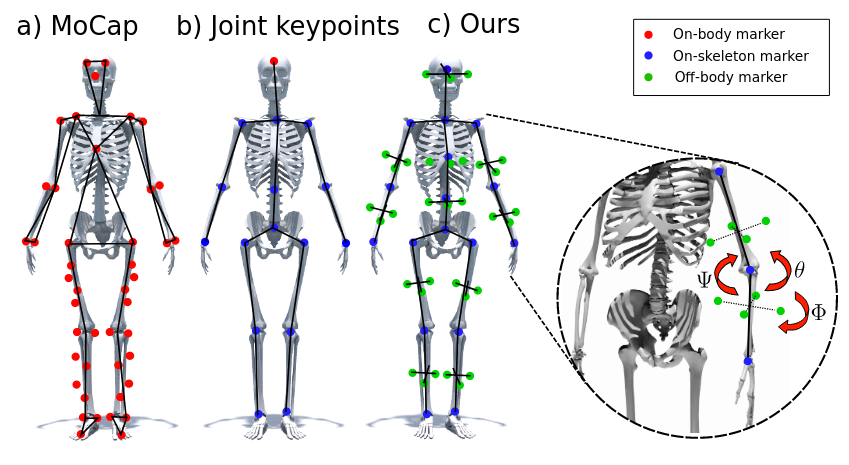
\includegraphics[width=0.8\linewidth]{figures/HPE/PoseExample.png}
    \caption[Example for human Pose estimation]{Example of a human pose captured with different methods. (a) A captured skeleton using MoCap which REPLACE_WE do not focus on in this report. (b) A traditional human skeleton representation. (c) A pose representation that includes the orientation of the joints as well as the bones as presented by Martin Fish and Ronald Clark\cite{KeypointOrientation}}
    \label{fig:pose_example}
\end{figure}

The second way to visualise a human pose is by using a 2D silhouette or 2D rectangles and shapes. These methods are also called contour-based methods. An example of contour-based methods was introduced by Yunheng Liu\cite{contourHPE}. Contour-based methods are often used in combination with a skeleton representation. The skeleton is used to determine the location of the joints, while the contour is used to determine the shape of the body. This is useful when the skeleton is not able to determine the shape of the body, for example, when the person is wearing a coat or a jacket. This is also used for some games developed by SilverFit.

Finally, the third way to represent a human pose is with a three-dimensional volume. This volume may be simple cylindrical shapes or a body mesh. A body mesh is a 3D representation of the body, which is made up of vertices and triangles. The three different representations of the human pose can be seen in Figure \ref{fig:pose_representation}.

\begin{figure}
    \centering
    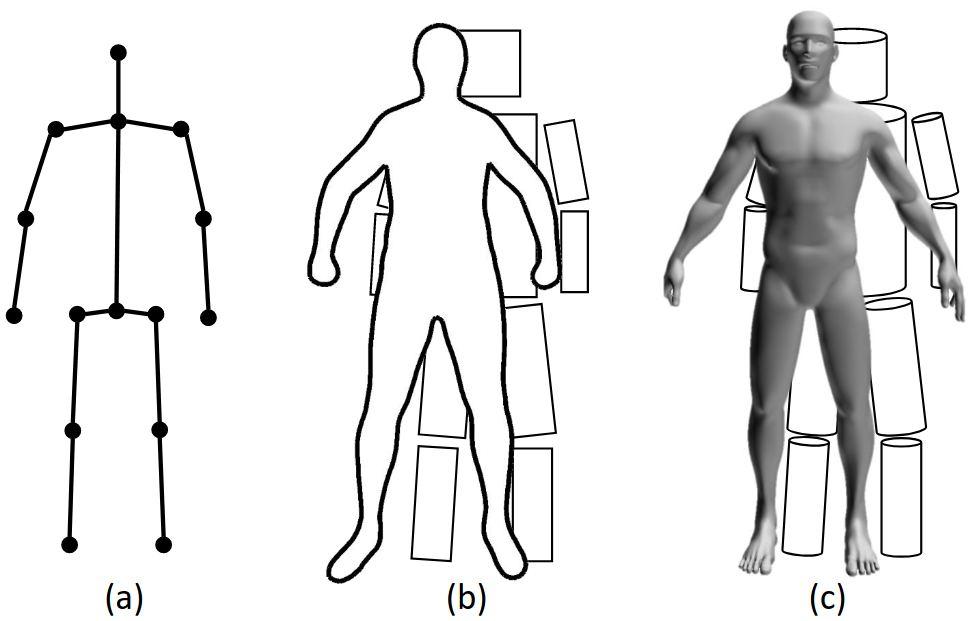
\includegraphics[width=0.8\linewidth]{figures/HPE/PoseRepresentation.png}
    \caption{Different representations of the human pose. (a) Skeleton representation. (b) Contour representation. (c) 3D volume representation. \cite{HPESurveyOriginal}}
    \label{fig:pose_representation}
\end{figure}

\subsection{Pose estimation data sources}

The pose of a human can be estimated from different types of data sources. The most common data source is RGB videos. RGB videos are any videos that are captured with normal cameras that record the color of the scene. The provided data can be either from a video or a stream of data or a still image. There is a large number of datasets that can be used to train and test pose estimation algorithms from RGB data. Some of the most common datasets are the MPII Human Pose Dataset\cite{MPII}, the COCO dataset\cite{Coco}, and HumanEva-I dataset\cite{HumanEva}.

Additionally, some datasets are captured with depth cameras. Depth cameras are cameras that can record the depth of the scene. This depth information can be used to improve the accuracy of the pose estimation. Some of the most common datasets that are captured with depth cameras are the MRI dataset\cite{mRI}, and the Human3.6M dataset\cite{h36m_pami}.

Finally, there are also methods of human pose estimation that use point clouds. Point clouds are a collection of points in space, which can be used to represent the shape of an object. Point clouds are often used in combination with RGB data. Some of the most common datasets that are captured with depth cameras are the SMMC-10 dataset\cite{SMMC10}, and the EVAL dataset\cite{EVAL}. However, any RGBD dataset can be used to train and test point cloud-based pose estimation algorithms if the camera intrinsics and extrinsic, such as the horizontal and vertical field of view, the focal point, and the depth units are known. With the knowledge of these parameters, the depth information can be converted to a point cloud and if the RGB data is in line with the depth data, the individual points can be colored accordingly.

Additionally, to the data that is provided, REPLACE_WE also differentiate between monocular and multi-modal data. Monocular data is data that is captured with a single camera. Multi-modal data is data that is captured with multiple cameras. The most common multi-modal data is stereo data, which is data that is captured with two cameras. The cameras are usually placed next to each other and are angled toward the same scene. This allows the cameras to capture the same scene from different angles and therefore improving the accuracy of the pose estimation. There are not many datasets for this type of data, but the most common one was captured by Waymo\cite{Waymo}.

However, RGB cameras are far more widely spread and generally cheaper than depth cameras. Hence, most methods use RGB cameras to estimate the pose of a human. However, since depth cameras can provide more detailed information about the scene, they can be used to improve the accuracy of the pose estimation and in this report, REPLACE_WE will mainly focus on monocular RGBD data.

\subsection{Depth cameras}

As mentioned earlier, human pose estimation generally works based on visual information. However, the use of depth cameras offers more detailed information about the scene, which can in turn improve the reliability of the pose estimation. Many different depth cameras function mainly on three different principles. Firstly there are stereo cameras. Stereo cameras try to calculate the depth of a scene similar to how human eyes work. Most of the time two lenses or cameras are placed or installed next to each other and are angled toward the same scene and then the depth of the scene is calculated by comparing the images captured by the two cameras. These cameras function on the spectrum of light which is visible to the human eye. 

The second type of depth camera is the time-of-flight camera. These cameras use a laser to calculate the depth of the scene. The laser is fired at the objects in the scene, and the time it takes for the laser to bounce back is used to calculate the distance between the camera and the object based on the theoretical time it would take light to travel. 

Finally, there are also structured light cameras. These cameras use a pattern of light that is known to the camera to calculate the depth structure of the scene. For both the time-of-flight and structured light cameras, the depth information is calculated based on the spectrum of light that is not visible to the human eye.

\subsection{Applications}

Human pose estimation finds application in many different fields. Here REPLACE_WE mention a few of the most common applications.

\subsubsection{Gaming and entertainment}

This is one of the most common applications of human pose estimation. Games can use human pose estimation in a way that makes the interaction between humans and computers very natural way. One of the games that kickstarted the use of depth cameras in games was the game Kinect by Microsoft. This game used a depth camera to track the movement of the player and used this information to control the game. This game was very successful and was used in many different games. 

\subsubsection{Autonomous Driving}

Autonomous driving has been in development ever since humans replaced horses with cars. However, the development of autonomous driving has been very slow. The main reason for this is that autonomous driving requires a lot of information about the environment. This information is usually provided by sensors that are installed in the car. However, sensors alone do not always suffice. In some cases, cars need to be able to estimate the pose of a human to make a decision. The posture of a human can be used to determine the action and therefore the future trajectory of the person. 

\subsubsection{Animation}

To emulate exactly human movements in animation, animators can either manually move the joints of a digital skeleton or they can use real human\footnote{Or animal} actors to provide the movement for them. The manual creation of realistic movement is oftentimes very time-consuming and also error-prone. Therefore, animators often use real human actors to provide the movement for them. This provides animators with a skeleton and movement which is accurate and does not include human error. In large production studios, this is often done with motion capture or MoCap. 

MoCap is a technique that uses cameras to capture the movement of a human actor. The cameras are placed around the actor and record the movement of the actor. The actor usually wears a suit that is covered with markers. These markers are used to determine the position of the actor. To reduce the amount of occlusion of the markers a large number of cameras are used. This allows the cameras to capture the movement of the actor from different angles. However, this also increases the price of development. In cases where MoCap is not a viable option, animators can use human pose estimation to estimate the pose of a human actor using cheaper RGB cameras or RGBD cameras.

\subsubsection{Healthcare}

One of the companies that develop games using human pose estimation is Silverfit. SilverFit uses both a skeletal representation as well as a contour representation of the human pose. Human pose estimation enables the game to provide the user with feedback on their posture. This feedback can be used to improve the posture of the user and also allows the physiotherapists to design specific exercises which engage the muscles that are not used enough.